\documentclass{standalone}
\usepackage{tikz}
\usetikzlibrary{patterns, positioning}

\begin{document}
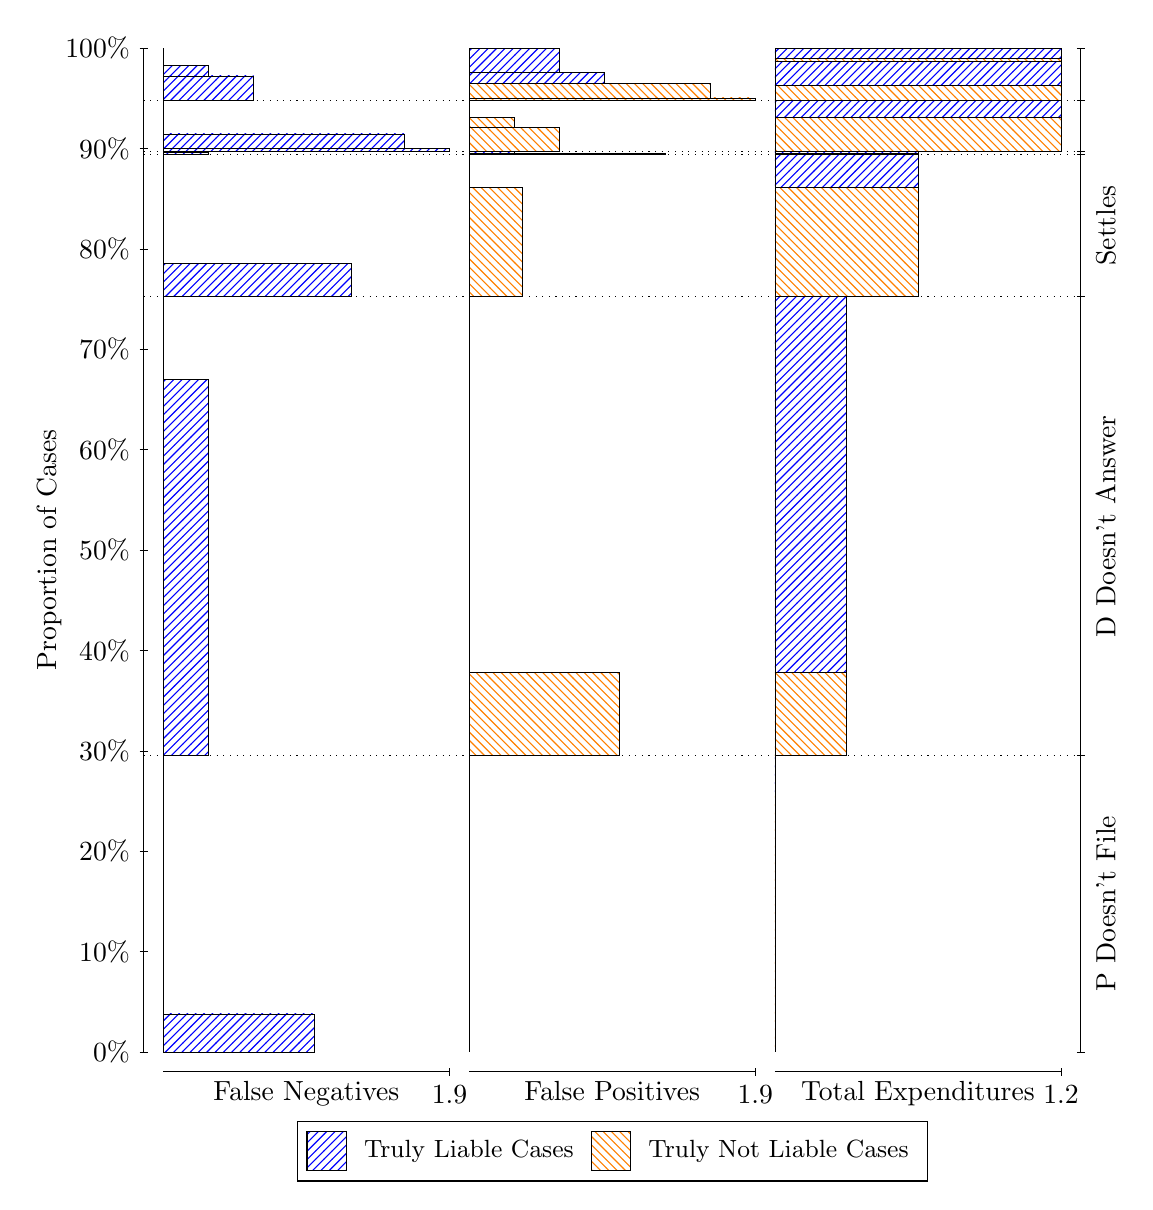
\begin{tikzpicture}
\draw[black, very thin] (1.5,1.75) -- (1.5,14.5);
\node[rotate=90, anchor=center] at (0.3, 8.125) {Proportion of Cases};
\draw[black, very thin] (1.45,1.75) -- (1.55,1.75);
\node[anchor=east] at (1.45, 1.75) {0\%};
\draw[black, very thin] (1.45,3.025) -- (1.55,3.025);
\node[anchor=east] at (1.45, 3.025) {10\%};
\draw[black, very thin] (1.45,4.3) -- (1.55,4.3);
\node[anchor=east] at (1.45, 4.3) {20\%};
\draw[black, very thin] (1.45,5.575) -- (1.55,5.575);
\node[anchor=east] at (1.45, 5.575) {30\%};
\draw[black, very thin] (1.45,6.85) -- (1.55,6.85);
\node[anchor=east] at (1.45, 6.85) {40\%};
\draw[black, very thin] (1.45,8.125) -- (1.55,8.125);
\node[anchor=east] at (1.45, 8.125) {50\%};
\draw[black, very thin] (1.45,9.4) -- (1.55,9.4);
\node[anchor=east] at (1.45, 9.4) {60\%};
\draw[black, very thin] (1.45,10.675) -- (1.55,10.675);
\node[anchor=east] at (1.45, 10.675) {70\%};
\draw[black, very thin] (1.45,11.95) -- (1.55,11.95);
\node[anchor=east] at (1.45, 11.95) {80\%};
\draw[black, very thin] (1.45,13.225) -- (1.55,13.225);
\node[anchor=east] at (1.45, 13.225) {90\%};
\draw[black, very thin] (1.45,14.5) -- (1.55,14.5);
\node[anchor=east] at (1.45, 14.5) {100\%};

\draw[black, very thin] (13.4,1.75) -- (13.4,14.5);
\draw[black, very thin] (13.35,1.75) -- (13.45,1.75);
\node[anchor=west] at (13.35, 1.75) {};
\draw[black, very thin] (13.35,5.5119) -- (13.45,5.5119);
\node[anchor=west] at (13.35, 5.5119) {};
\draw[black, very thin] (13.35,11.345) -- (13.45,11.345);
\node[anchor=west] at (13.35, 11.345) {};
\draw[black, very thin] (13.35,13.148) -- (13.45,13.148);
\node[anchor=west] at (13.35, 13.148) {};
\draw[black, very thin] (13.35,13.191) -- (13.45,13.191);
\node[anchor=west] at (13.35, 13.191) {};
\draw[black, very thin] (13.35,13.835) -- (13.45,13.835);
\node[anchor=west] at (13.35, 13.835) {};
\draw[black, very thin] (13.35,14.5) -- (13.45,14.5);
\node[anchor=west] at (13.35, 14.5) {};

\draw[black, very thin, pattern color=blue, pattern=north east lines] (1.75,1.75) rectangle (3.6623,2.2345);
\draw[black, very thin, pattern color=orange, pattern=north west lines] (1.75,2.2345) rectangle (1.75,5.5119);
\draw[black, very thin, pattern color=blue, pattern=north east lines] (1.75,5.5119) rectangle (2.3237,10.289);
\draw[black, very thin, pattern color=orange, pattern=north west lines] (1.75,10.289) rectangle (1.75,11.345);
\draw[black, very thin, pattern color=blue, pattern=north east lines] (1.75,11.345) rectangle (4.1404,11.761);
\draw[black, very thin, pattern color=orange, pattern=north west lines] (1.75,11.761) rectangle (1.75,13.148);
\draw[black, very thin, pattern color=blue, pattern=north east lines] (1.75,13.148) rectangle (2.3237,13.18);
\draw[black, very thin, pattern color=orange, pattern=north west lines] (1.75,13.18) rectangle (1.75,13.191);
\draw[black, very thin, pattern color=blue, pattern=north east lines] (1.75,13.191) rectangle (5.3833,13.223);
\draw[black, very thin, pattern color=blue, pattern=north east lines] (1.75,13.223) rectangle (4.8096,13.411);
\draw[black, very thin, pattern color=orange, pattern=north west lines] (1.75,13.411) rectangle (1.75,13.835);
\draw[black, very thin, pattern color=blue, pattern=north east lines] (1.75,13.835) rectangle (2.8974,14.146);
\draw[black, very thin, pattern color=blue, pattern=north east lines] (1.75,14.146) rectangle (2.3237,14.281);
\draw[black, very thin, pattern color=orange, pattern=north west lines] (1.75,14.281) rectangle (1.75,14.5);
\draw[black, very thin, pattern color=orange, pattern=north west lines] (5.6333,1.75) rectangle (5.6333,5.0274);
\draw[black, very thin, pattern color=blue, pattern=north east lines] (5.6333,5.0274) rectangle (5.6333,5.5119);
\draw[black, very thin, pattern color=orange, pattern=north west lines] (5.6333,5.5119) rectangle (7.5456,6.5672);
\draw[black, very thin, pattern color=blue, pattern=north east lines] (5.6333,6.5672) rectangle (5.6333,11.345);
\draw[black, very thin, pattern color=orange, pattern=north west lines] (5.6333,11.345) rectangle (6.3026,12.732);
\draw[black, very thin, pattern color=blue, pattern=north east lines] (5.6333,12.732) rectangle (5.6333,13.148);
\draw[black, very thin, pattern color=orange, pattern=north west lines] (5.6333,13.148) rectangle (8.1193,13.159);
\draw[black, very thin, pattern color=blue, pattern=north east lines] (5.6333,13.159) rectangle (6.207,13.191);
\draw[black, very thin, pattern color=orange, pattern=north west lines] (5.6333,13.191) rectangle (6.7807,13.49);
\draw[black, very thin, pattern color=orange, pattern=north west lines] (5.6333,13.49) rectangle (6.207,13.615);
\draw[black, very thin, pattern color=blue, pattern=north east lines] (5.6333,13.615) rectangle (5.6333,13.835);
\draw[black, very thin, pattern color=orange, pattern=north west lines] (5.6333,13.835) rectangle (9.2667,13.868);
\draw[black, very thin, pattern color=orange, pattern=north west lines] (5.6333,13.868) rectangle (8.693,14.054);
\draw[black, very thin, pattern color=blue, pattern=north east lines] (5.6333,14.054) rectangle (7.3544,14.189);
\draw[black, very thin, pattern color=blue, pattern=north east lines] (5.6333,14.189) rectangle (6.7807,14.5);
\draw[black, very thin, pattern color=orange, pattern=north west lines] (9.5167,1.75) rectangle (9.5167,5.0274);
\draw[black, very thin, pattern color=blue, pattern=north east lines] (9.5167,5.0274) rectangle (9.5167,5.5119);
\draw[black, very thin, pattern color=orange, pattern=north west lines] (9.5167,5.5119) rectangle (10.425,6.5672);
\draw[black, very thin, pattern color=blue, pattern=north east lines] (9.5167,6.5672) rectangle (10.425,11.345);
\draw[black, very thin, pattern color=orange, pattern=north west lines] (9.5167,11.345) rectangle (11.333,12.732);
\draw[black, very thin, pattern color=blue, pattern=north east lines] (9.5167,12.732) rectangle (11.333,13.148);
\draw[black, very thin, pattern color=orange, pattern=north west lines] (9.5167,13.148) rectangle (11.333,13.159);
\draw[black, very thin, pattern color=blue, pattern=north east lines] (9.5167,13.159) rectangle (11.333,13.191);
\draw[black, very thin, pattern color=orange, pattern=north west lines] (9.5167,13.191) rectangle (13.15,13.615);
\draw[black, very thin, pattern color=blue, pattern=north east lines] (9.5167,13.615) rectangle (13.15,13.835);
\draw[black, very thin, pattern color=orange, pattern=north west lines] (9.5167,13.835) rectangle (13.15,14.021);
\draw[black, very thin, pattern color=blue, pattern=north east lines] (9.5167,14.021) rectangle (13.15,14.332);
\draw[black, very thin, pattern color=orange, pattern=north west lines] (9.5167,14.332) rectangle (13.15,14.365);
\draw[black, very thin, pattern color=blue, pattern=north east lines] (9.5167,14.365) rectangle (13.15,14.5);
\draw[black, dotted] (1.5,5.5119) -- (13.4,5.5119);
\draw[black, dotted] (1.5,11.345) -- (13.4,11.345);
\draw[black, dotted] (1.5,13.148) -- (13.4,13.148);
\draw[black, dotted] (1.5,13.191) -- (13.4,13.191);
\draw[black, dotted] (1.5,13.835) -- (13.4,13.835);
\draw[black, very thin] (1.75,1.5) -- (5.3833,1.5);
\node[anchor=north] at (3.5667, 1.5) {False Negatives};
\draw[black, very thin] (5.3833,1.45) -- (5.3833,1.55);
\node[anchor=north] at (5.3833, 1.45) {1.9};

\draw[black, very thin] (5.6333,1.5) -- (9.2667,1.5);
\node[anchor=north] at (7.45, 1.5) {False Positives};
\draw[black, very thin] (9.2667,1.45) -- (9.2667,1.55);
\node[anchor=north] at (9.2667, 1.45) {1.9};

\draw[black, very thin] (9.5167,1.5) -- (13.15,1.5);
\node[anchor=north] at (11.333, 1.5) {Total Expenditures};
\draw[black, very thin] (13.15,1.45) -- (13.15,1.55);
\node[anchor=north] at (13.15, 1.45) {1.2};

\node[black, centered, rotate=90] at (13.72, 3.6309) {P Doesn't File};
\node[black, centered, rotate=90] at (13.72, 8.4283) {D Doesn't Answer};
\node[black, centered, rotate=90] at (13.72, 12.246) {Settles};




\draw (7.449999999999999,1.5) node[draw=none] (baseCoordinate) {};
\begin{scope}[align=center]
        \matrix[scale=0.5, draw=black, below=0.5cm of baseCoordinate, nodes={draw}, column sep=0.1cm]{
            \node[rectangle, draw, minimum width=0.5cm, minimum height=0.5cm, pattern=north east lines, pattern color=blue] {}; &
            \node[draw=none, font=\small] (B) {Truly Liable Cases}; &
            \node[rectangle, draw, minimum width=0.5cm, minimum height=0.5cm, pattern=north west lines, pattern color=orange] {}; &
            \node[draw=none, font=\small] (B) {Truly Not Liable Cases}; \\
            };
\end{scope}

\end{tikzpicture}
\end{document}